\chapter{Datasets}

\begin{quote}
    In this chapter, we first give a short background on the standardisation of datasets and evaluation procedures in the field of MIR. Then, we give a more detailed description of the datasets that were used for the experiments in this thesis.
\end{quote}

We used the MagnaTagATune dataset and Million Song Dataset \cite{Bertin-Mahieux2011} for pre-training and evaluation.

For the transfer learning experiments, we pre-train CLMR on the Million Song Dataset, fault-filtered GTZAN \cite{tzanetakis2002musical,sturm2013gtzan}, McGill Billboard \cite{burgoyne_billboard} and Free Music Archive \cite{fma_dataset} datasets.
We subsequently perform linear evaluation of the self-supervised learned representations on the MagnaTagATune dataset.

\section{MIREX}
There are several benchmark datasets that are used to evaluate music classification algorithms with.
One of the first attempts to unify datasets and evaluation procedures for music (classification) algorithms is MIREX: the Music Information Retrieval Evaluation eXchange.
This `exchange' was started as a platform to evaluate newly published algorithms on many tasks in the field of MIR.
The MIR tasks range from chord recognition, music key detection, audio fingerprinting to music classification.
Along with the unification of evaluation procedures, it has also produced standard datasets to benchmark algorithms with.
For the task of music classification, the MagnaTagATune dataset \cite{law2009evaluation} is often used.
For chord recognition, the Billboard dataset is regarded as a standard dataset \cite{burgoyne_billboard}.


\section{MagnaTagATune Dataset}
The MagnaTagATune dataset was compiled by crowdsourcing tags from a game called `TagATune' using music from the Magnatune label.
For the MagnaTagATune dataset, we used the original, MIREX 2009 version, consisting of 25\,863 songs, and the same dataset split, so that we can compare our results with previous work easily \cite{pons_end--end_2017, lee2018samplecnn, dieleman_feature_learning}.
It should be noted that this original version contains tag labels that are synonymous, e.g., `female', `woman', `no vocal', `no voice' and also contains tracks that do not have any labels. The top-50 tags in the MagnaTagATune dataset are shown in Table \ref{tab:magnatagatune_tags}.

The distribution of the number of fragments per class is skewed: there are more fragments containing guitar and classical tag attributes than `country' or `harp' attributes. A possible consequence of this class imbalance, is that CLMR learns representations that separate, e.g., `guitar' music and `flute' music well, but it is harder to learn representations that separate `country' music from `choral' music.


\begin{figure}
    \centering
    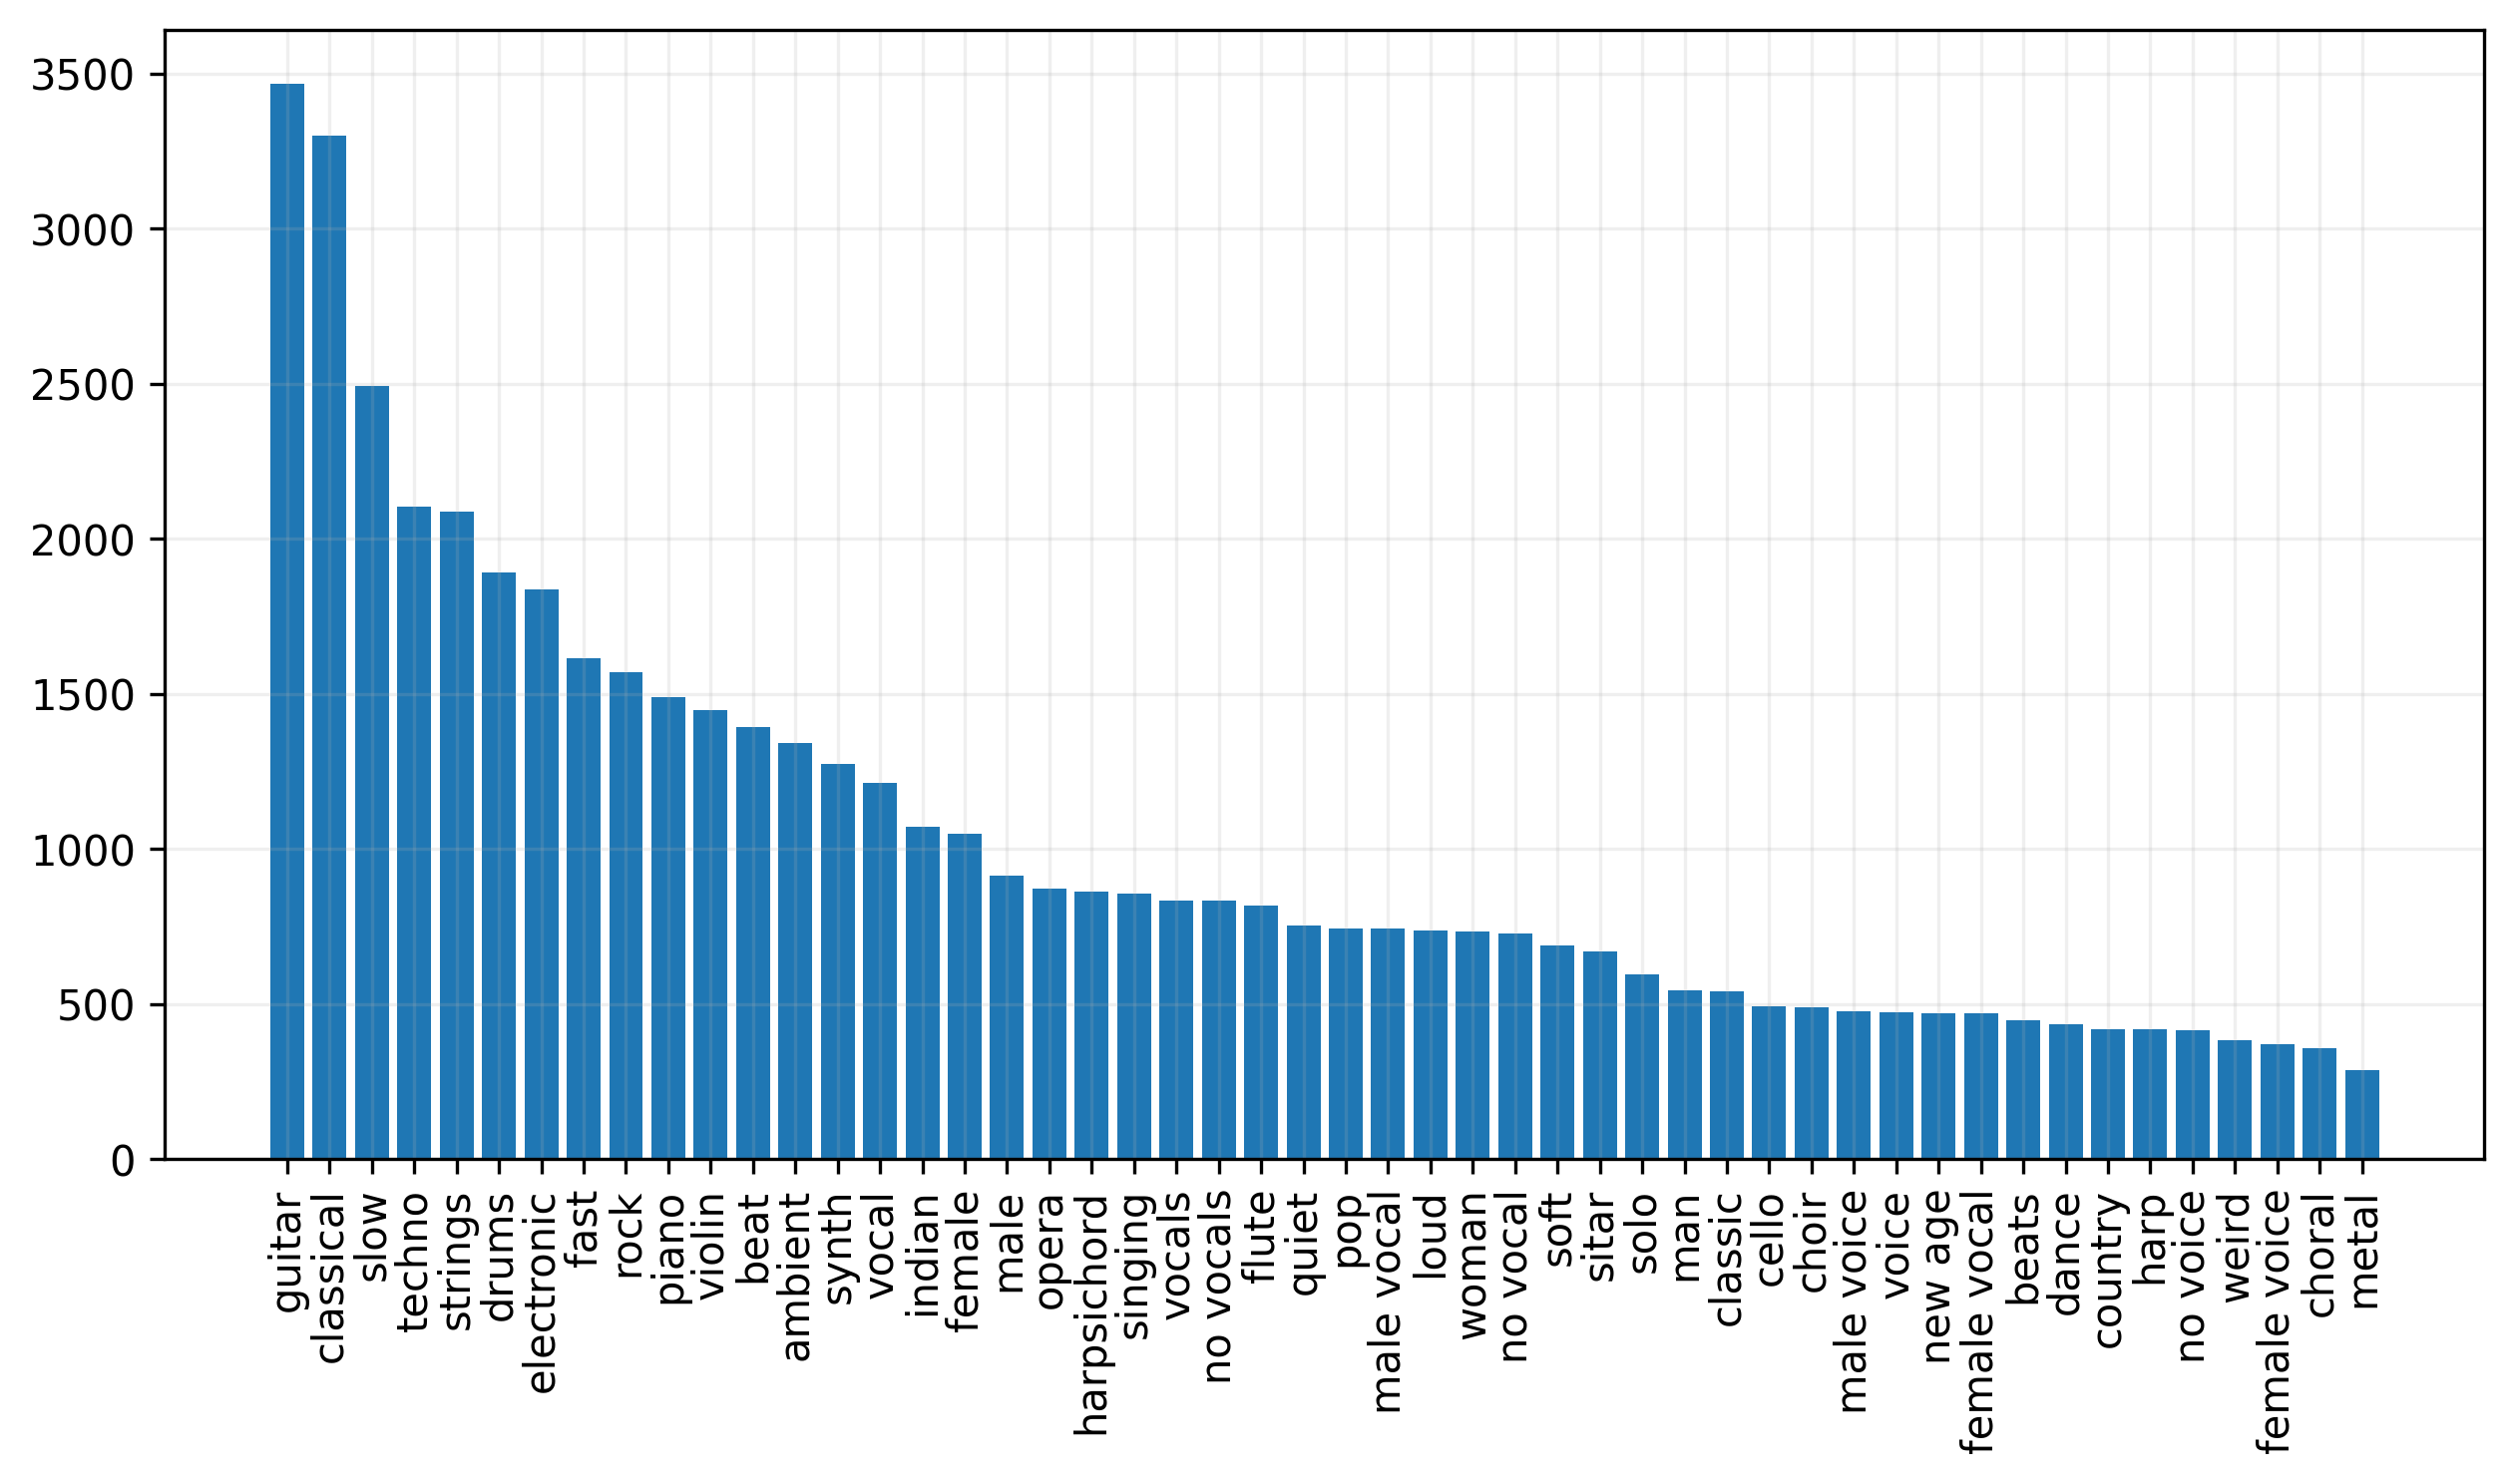
\includegraphics[width=\columnwidth]{figs/tag_stats_magnatagatune.png}
    \caption{Distribution of tags of the MagnaTagATune dataset}
    \label{fig:tag_stats_magnatagatune}
\end{figure}


\begin{table}[t]
    \centering
    \begin{tabular}{lll}\toprule
        guitar  & classical & slow \\
        techno & strings & drums \\
        electronic & rock & fast \\
        piano & ambient & beat \\
        violin & vocal & synth \\
        female & indian & opera \\
        male & singing & vocals \\
        no vocals & harpsichord & loud \\
        quiet & flute & woman \\
        male vocal & no vocal & pop \\
        soft & sitar & solo \\
        man & classic & choir \\
        voice & new age & dance \\
        male voice & female vocal & beats \\
        harp & cello & no voice \\
        weird & country & metal \\
        female voice & choral & \\                 
        \bottomrule
    \end{tabular}
    \caption{50 most popular tags in the MagnaTagATune dataset}
    \label{tab:magnatagatune_tags}
\end{table}



\section{Million Song Dataset}
The Million Song Dataset consists of 1 million audio features and metadata of contemporary pop songs.
It is commonly used for benchmarking on a larger scale.
These features were compiled by The Echo Nest, a music data company that has since been purchased by Spotify.
While they provide the audio features that are computed using their proprietary algorithms, the raw audio data is not provided due to the infringement of copyright when published freely and publicly.

Since this thesis uses raw audio to train and evaluate the CLMR model on, it was a challenge to obtain the raw audio of the contempory pop songs.
Originally, it could be obtained by accessing 30-second fragments using the internal IDs matched with those from the `7 digital' music service.
\footnote{\url{7digital.com}}
Since it does not provide this service anymore, we had to obtain the dataset from a another MIR research group that archived the 7digital fragments.
\footnote{We would like to thank Jongpil Lee from the Korea Advanced Institute of Science and Technology for providing us access to their server to retrieve the 30-second raw audio fragments.}

The Million Song Dataset's tags were compiled by cross-referencing it with the crowdsourced Last.fm dataset \cite{Bertin-Mahieux2011}. Similar to the MagnaTagATune dataset, we use only tracks that were annotated with tags from the set of top-50 most popular tags. This results in $241,904$ unique songs.

The tags for the Million Song Dataset are more overlapping, e.g., `rock' and `classic rock', and contain more semantic tags, e.g., `beautiful', `happy' and `sad', which are arguably harder to linearly separate when fine-tuning the linear classifier.
The top-50 tags are shown in Table \ref{tab:msd_tags}. Similar to the MagnaTagATune dataset, the classes are also imbalanced in this dataset. 
The `rock' attribute is overrepresented in the dataset.
While we did not correct for this imbalance, we reckon it has a similar effect on the learned representations as described earlier for the MagnaTagATune dataset.


\begin{figure}
    \centering
    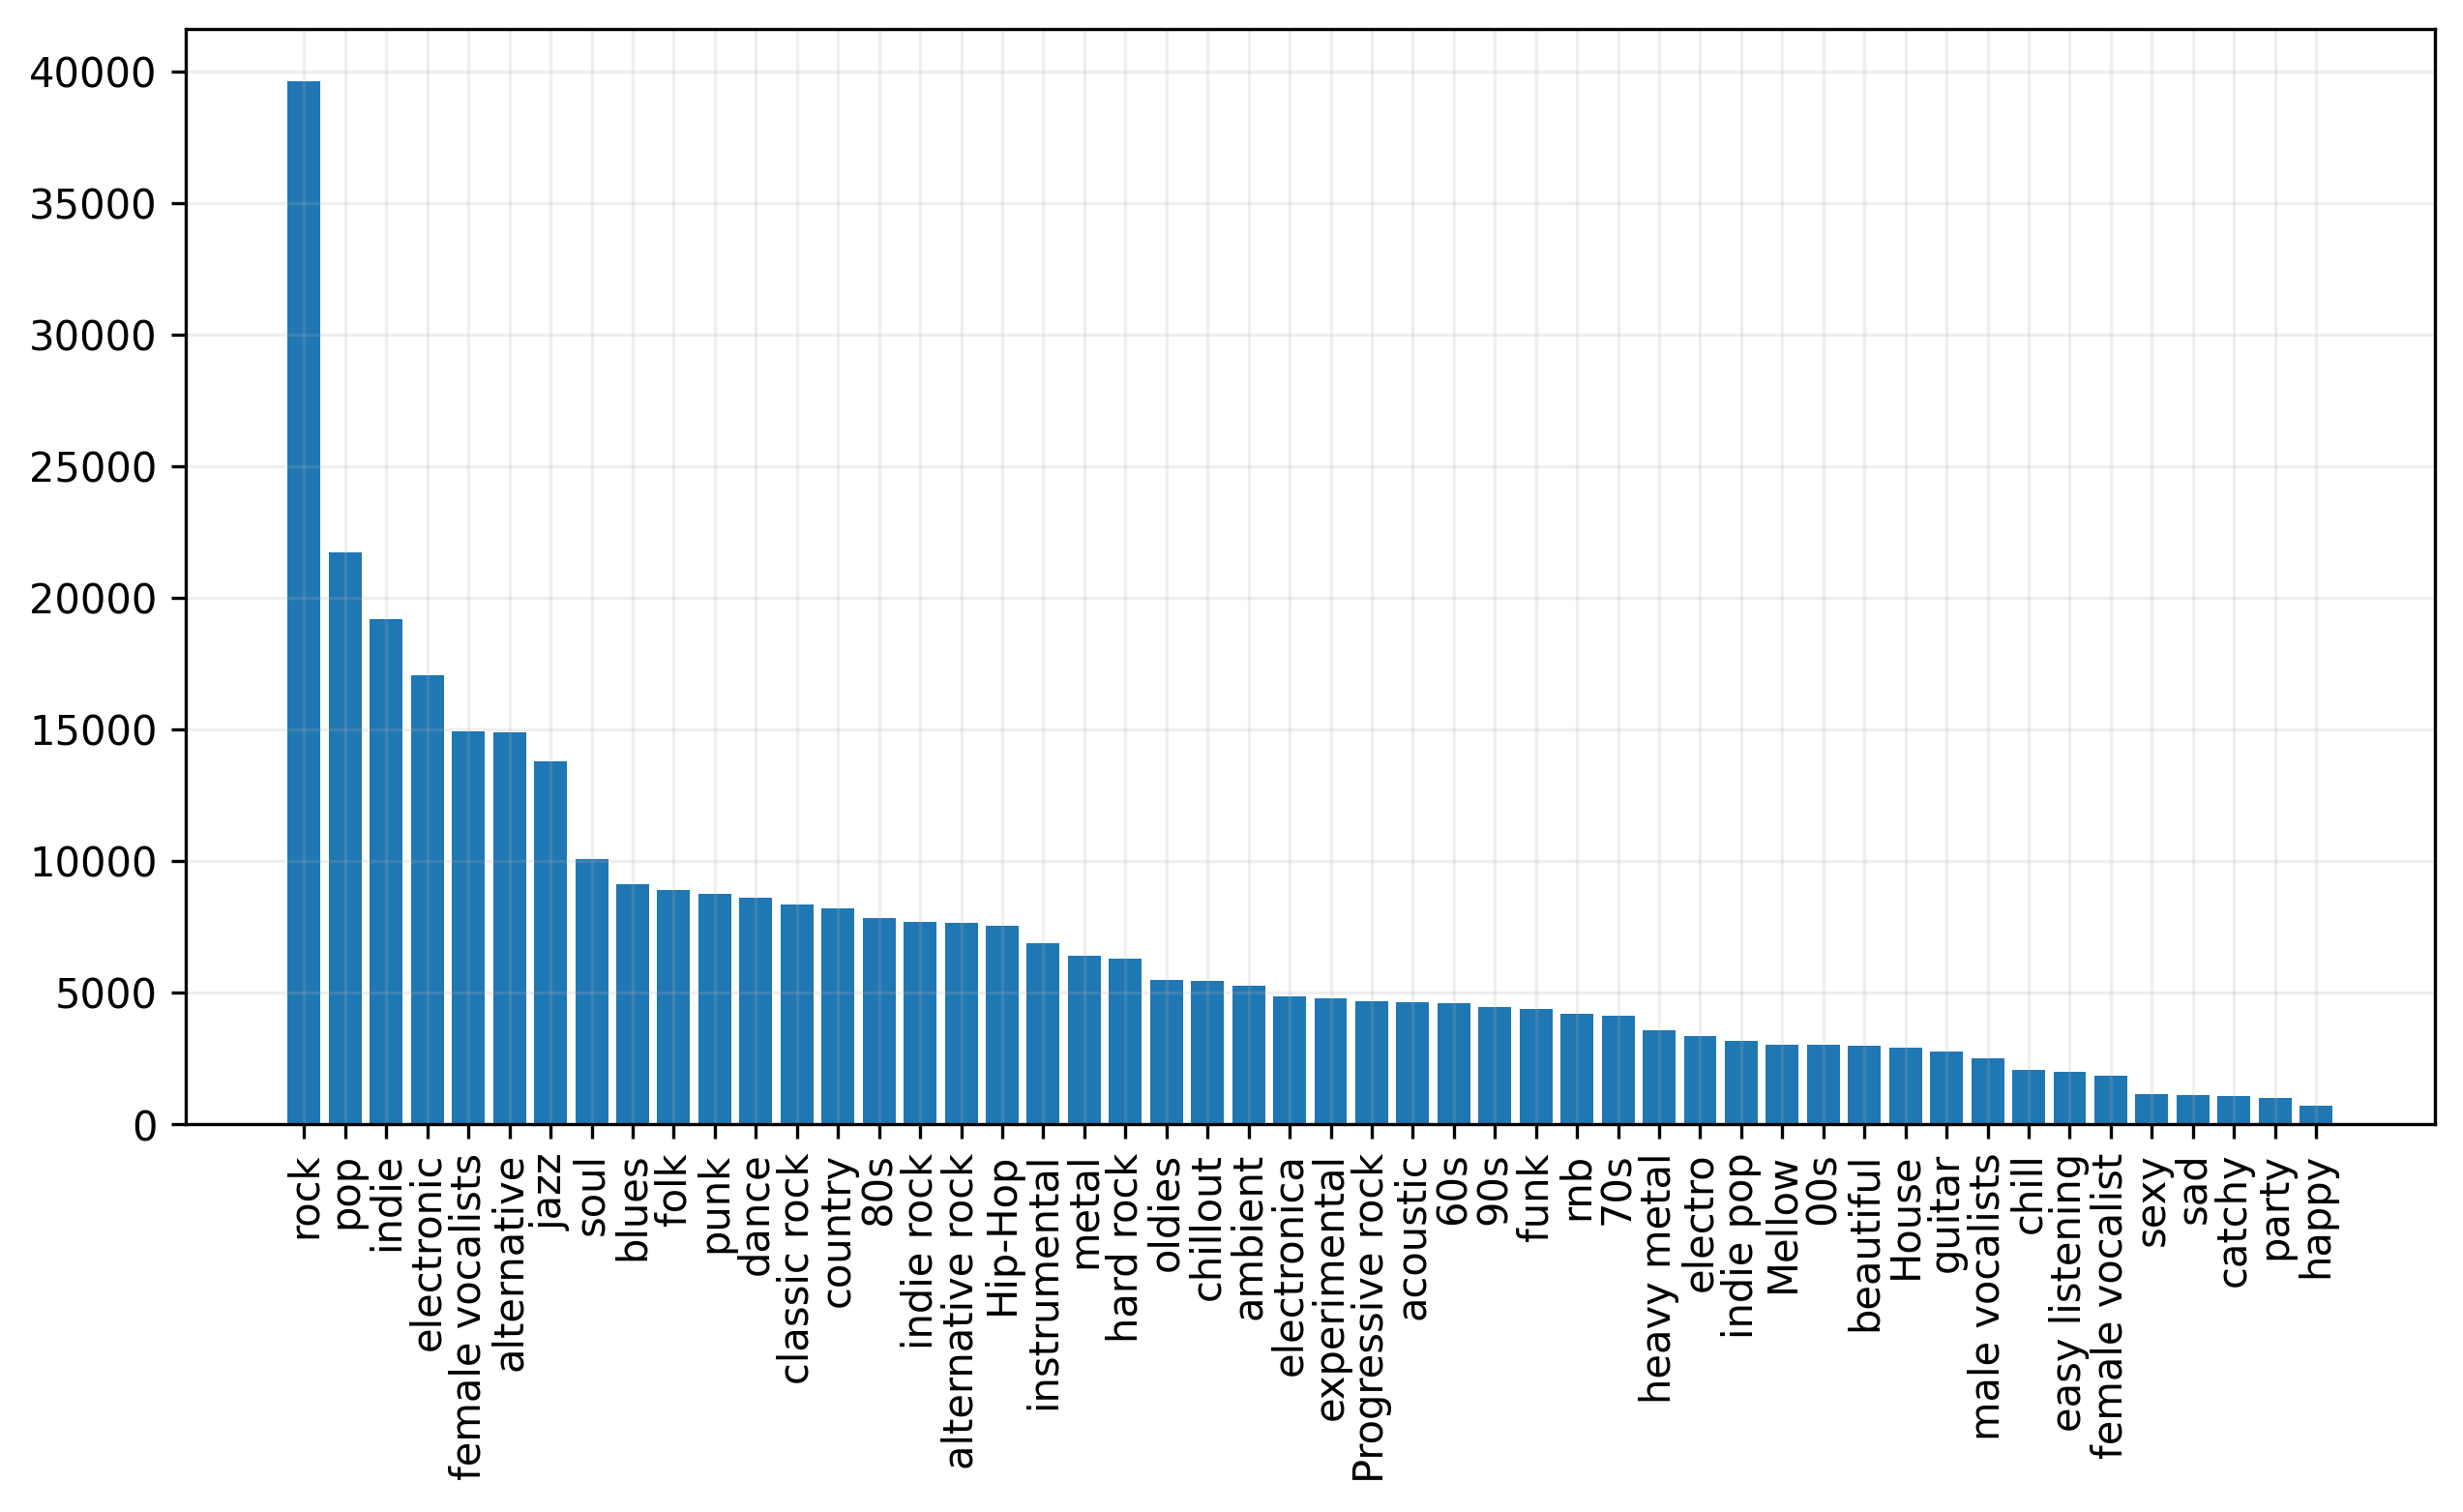
\includegraphics[width=\columnwidth]{figs/tag_stats_msd.png}
    \caption{Distribution of tags of the Million Song Dataset}
    \label{fig:tag_stats_msd}
\end{figure}


\begin{table}[t]
    \centering
    \begin{tabular}{lll}\toprule
        rock & pop & alternative \\
        indie & electronic & female vocalists \\
        dance & 00s & alternative rock \\
        jazz & beautiful & metal \\
        chillout & male vocalists & classic rock \\
        soul & indie rock & mellow \\
        electronica & 80s & folk \\
        90s & chill & instrumental \\
        punk & oldies & blues \\
        hard rock & ambient & acoustic \\
        experimental & female vocalist & guitar \\
        hip-hop & 70s & party \\
        country & easy listening & sexy \\
        catchy & funk & electro \\
        heavy metal & progressive rock & 60s \\
        rnb & indie pop & sad \\
        house & happy & \\
        \bottomrule
    \end{tabular}
    \caption{50 most popular tags in the Million Song Dataset}
    \label{tab:msd_tags}
\end{table}



% Like the other studies, we use average tag-wise ROC-AUC and PR-AUC scores as evaluation metrics, which are global measures indicating how well the classifier ranks segments given a tag.
% PR-AUC is calculated in addition to ROC-AUC because ROC-AUC scores can be over-optimistic for imbalanced datasets like Magna\-Tag\-A\-Tune.


\section{Transfer Learning Datasets}
\subsection{McGill Billboard Dataset}
From the McGill Billboard dataset, we use 461 audio files of contemporary pop songs for training.
While this dataset is most often used for evaluating chord recognition algorithms, we use the audio solely for self-supervised pre-training. The audio is only used for self-supervised pre-training.

\subsection{Free Music Archive}
Similarly, we use the Free Music Archive dataset, consisting of 22\,413 unique multi-labeled songs for the `medium' version, 

\subsection{GTZAN}
The fault-filtered GTZAN dataset contains 930 segments of 30 seconds, each having a single label denoting its genre \cite{Sturm2015, tzanetakis2002musical}. The dataset is made up of 10 genres: classical, country, disco, hip-hop, jazz, rock, blues, reggae, pop and metal. The audio is again only used for self-supervised pre-training.

